% !TeX root = ../handout.tex

\section{Einleitung und Motivation}

Seit über 40 Jahren ist das Konzept des \emph{Data Sharing} Bestandteil der Forschung.
Data Sharing beschreibt dabei den Prozess, bei dem Dritten Zugriff auf Daten gewährt wird, auf welche diese sonst keinen Zugriff hätten (vgl. Beispiel aus \autoref{fig:example-data-donation}).
Das Internet und die Einführung von Smartphones ermöglicht es, nahezu sofort Daten zu erhalten und weiter zu verteilen.
Auch im betrieblichen Kontext sind Daten essenziell.
Sie sind für nahezu alle Geschäftsprozesse notwendig, sodass sie sich vom \enquote{Nebenprodukt} zur \emph{strategischen Ressource} entwickelten~\cite{mollerIndustrialDataEcosystems2024}.
Es gibt viele Bedenken beim Teilen von Daten, wie bspw. der Angst vor unberechtigter Weitergabe (Geschäftsgeheimnisse), Missbrauch von Daten oder Kontrollverlust~\cite{mollerIndustrialDataEcosystems2024}.
Eine Vertrauensbasis fehlt, um ein multi"=laterales Datennetz zu spannen.

\begin{figure}
    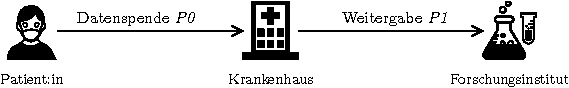
\includegraphics[width=\textwidth]{./assets/example_horizontal.drawio.pdf}
    \caption{Beispiel für Data Sharing: Datenspende zur Weiterverwendung für Forschung}
    \label{fig:example-data-donation}
\end{figure}

Um Daten zwischen verschiedenen Akteuren zu teilen, ist oft eine Datenintegration, bspw. via \emph{Extract, Transform, Load} (ETL) notwendig, welche essenziell für den Erfolg von Geschäftsprozessen ist.
Solche Integrationen sind oftmals aufwendig und zeitintensiv.
Nach Abschluss haben sich die Modelle und Projekte teilweise schon wieder verändert, sodass Inkonsistenzen und hohe Kosten durch die wiederholte Ausführung von Schritten entstehen.
Durch hohe Kosten liegt die Einstiegsbarriere für neue Akteure hoch, wodurch die Zugänglichkeit und Innovationsfähigkeit eingeschränkt wird.
Ein effizientes, schnelles und günstiges Verfahren, welches für alle zugänglich, sowie stets verfügbare und konsistente Daten schafft, ist notwendig.

Da Daten als wertvolles Wirtschaftsgut zu betrachten ist, werden diese \emph{en masse} gespeichert.
Aufgrund von mangelndem Vertrauen und dadurch mangelnder Kooperation, werden dieselben Daten mehrfach an verschiedenen Orten gespeichert.
Da Nutzende sich oft ihre Daten und Privatsphäre nicht kontrollieren können, werden diese oft nur zurückhaltend geteilt.
Somit entstehen mehrere große Datensilos, welche inkonsistent und teils veraltete Daten enthalten.
Wünschenswert wäre die Verfügbarkeit von aktuellen, konsistenten Daten sowie die Kombination Datenschutz und Zugriffskontrolle (vgl. Datensouveränität).

An dieser Stelle setzt das Konzept der \emph{Data Spaces} an. Dieses adressiert diese Probleme, in dem es einen multi"=lateralen, sicheren und vertrauenswürdigen Datenaustausch ermöglicht, welches Datensouveränität garantiert~\cite{mollerIndustrialDataEcosystems2024}.
Der Begründer des \emph{World Wide Web}s, Tim Berners"=Lee, stellte dazu 2016 den Solid"=Standard (ehem. \emph{Social Linked Data}) vor, welches ein Fundament für offene, dezentralisierte Netzwerke für einen souveränen Datenaustausch ermöglichen möchte~\cite{mecklerWebLinkedData2023}.
